\documentclass[12pt]{article}
% Basic packages
\usepackage[utf8]{inputenc}   % UTF-8 encoding
\usepackage{geometry}          % Page margins
\usepackage{setspace}          % Double spacing
\usepackage{amsmath, amssymb} % Math symbols
\usepackage{graphicx}         % Include images
\usepackage{booktabs}         % Nice tables
\usepackage{enumitem}         % Custom lists
\usepackage{cancel}
\usepackage{float}

% Page setup: 1-inch margins
\geometry{
  letterpaper,
  margin=1in
}

% Double spacing
\doublespacing{}

% START OF DOCUMENT %
\begin{document}

\begin{center}
    {\textbf{Johnny A. Rojas \& Aiden Sitorus, George Nicacio, Jeremiah
        Hasibuan, Matthew Miller}}\\
    {\Large \textbf{A LAB REPORT ON BALMER SERIES AND RYDBERG CONSTANT}}
\end{center}


\section{Theory}
The Balmer Series, formalized in 1885 by Johann Jakob Balmer, is a mathematical
model describing the quantized relationship between the spectral emission lines of
a hydrogen atom and the principal quantum number of the electron's initial energy
state. This relationship is governed by a proportionality constant $R$, known as
the Rydberg constant, and is expressed as:

\begin{align*}
    \frac{1}{\lambda} = R \left( \frac{1}{2^2} - \frac{1}{n^2} \right)
\end{align*}

where:
\begin{itemize}
    \item $\lambda$ is the wavelength of the emission line (in meters),
    \item $R$ is the Rydberg constant ($R \approx 1.097 \times 10^7 \ \mathrm{m^{-1}}$),
    \item $n$ is the principal quantum number of the initial state ($n > 2$).
\end{itemize}

This expression specifically describes electron transitions in which the final
state of the hydrogen atom corresponds to $n_f = 2$, meaning the electron falls
to the second energy level. The emitted photon's wavelength falls within the
visible spectrum, producing the characteristic colored lines of the Balmer Series.
Given the Rydberg constant, this formula allows us to predict the wavelengths of
the spectral emission lines by rearranging the expression accordingly.

To experimentally validate this relationship, one can measure the wavelengths of
the spectral lines from a hydrogen source using a diffraction grating setup. The
governing relationship for a diffraction grating is:

\begin{align*}
    m * \lambda = d * \sin(\theta)
\end{align*}

where:
\begin{itemize}
    \item $\theta$ is the angle of diffraction relative to the incident beam (in degrees),
    \item $m$ is the order of interference,
    \item $d$ is the grating spacing --- the distance between two consecutive slits (in meters).
\end{itemize}

Since $d$ is not directly measured, a mercury light source is first used to
calibrate the grating. Mercury produces well-known spectral lines whose wavelengths
are established, allowing us to solve for $d$ experimentally. Once $d$ is
determined, the same grating is used with the hydrogen source to measure the
diffraction angles of its spectral lines, from which the corresponding wavelengths
are calculated. Finally, these measured wavelengths are substituted back into the
Balmer Series equation to compute an experimental value of the Rydberg constant $R$,
which can then be compared to the accepted theoretical value.
\section{Conclusion}
In Activity 1, a mercury light source was used to experimentally determine the
grating spacing $d$ of the diffraction grating through calibration. Using the
NIST reference wavelengths for the red, green/cyan, and violet spectral lines of
mercury alongside their measured diffraction positions, individual values of $d$
were calculated for each line and averaged, yielding:

\begin{align*}
    \bar{N} = 989.26 \ \text{lines/mm} \quad \Longrightarrow \quad
    \bar{d} = 1.0109 \times 10^{-6} \ \text{m}
\end{align*}

This calibrated grating spacing was then used in Activity 2 to measure the
wavelengths of the hydrogen spectral lines. The diffraction angles for the red
($n = 3$), green ($n = 4$), and violet ($n = 5$) transitions were recorded, and
the corresponding wavelengths were calculated using $\lambda = d\sin(\theta)/m$.
These experimental wavelengths were substituted into the Balmer Series equation
to compute an individual Rydberg constant $R$ for each spectral line, summarized
in the table below:

\begin{center}
\begin{tabular}{lccc}
\hline
\textbf{Color} & \textbf{$n$} & \textbf{$\lambda_{\text{exp}}$ (m)} & \textbf{$R_{\text{measured}}$ (m$^{-1}$)} \\
\hline
Red    & 3 & $6.803 \times 10^{-7}$ & $1.058 \times 10^{7}$ \\
Green  & 4 & $5.414 \times 10^{-7}$ & $0.985 \times 10^{7}$ \\
Violet & 5 & $4.611 \times 10^{-7}$ & $1.033 \times 10^{7}$ \\
\hline
\end{tabular}
\end{center}

Averaging these values yields an experimental Rydberg constant of:

\begin{align*}
    R_{\text{exp}} = 1.0255 \times 10^{7} \ \text{m}^{-1}
\end{align*}

Comparing this to the accepted value of $R = 1.0970 \times 10^{7} \ \text{m}^{-1}$,
the percent error is:

\begin{align*}
    \% \text{ Error} = \frac{|R_{\text{exp}} - R|}{R} \times 100 = 6.52\%
\end{align*}

This level of agreement validates the Balmer Series relationship within the
bounds of experimental uncertainty. The observed discrepancy is likely attributable
to systematic errors in the data collection process, particularly in the visual
identification of the spectral line positions on the ruler, which introduces
uncertainty in the measured $x$ values and consequently in the computed angles
$\theta$. Additionally, any slight misalignment of the grating or the light source
relative to the optical axis would propagate through both activities and contribute
to the final error in $R$.
\section{Question}

\begin{figure}[H]
  \centering
  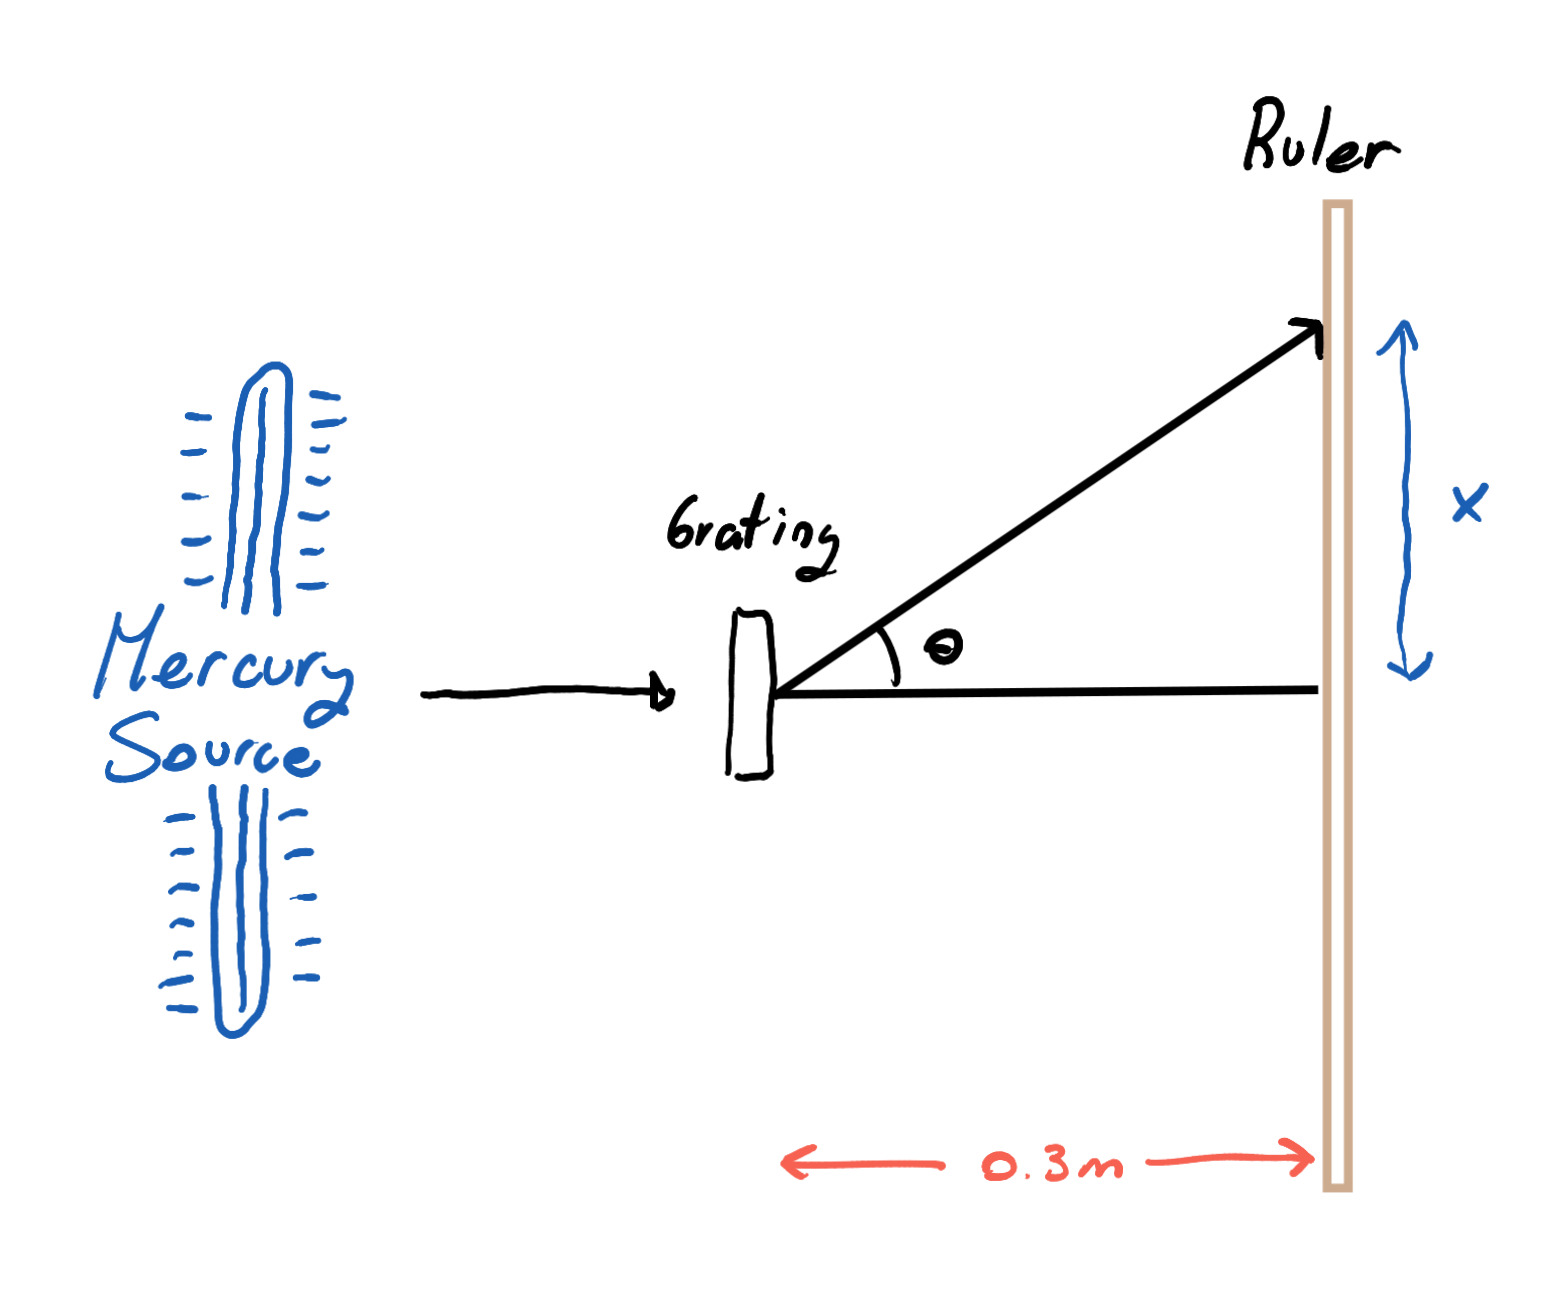
\includegraphics[width=0.5\textwidth]{Tables/image.jpeg}
\end{figure}

\begin{enumerate}
    \item Set up the mercury light source in front of the diffraction grating
    and position a ruler perpendicular to the incoming light at a fixed
    distance of $L = 0.3$ m from the grating.
    \item For each visible spectral line of mercury (red, green/cyan, and
    violet), record the positions of the diffracted line on both the right
    and left sides of the central beam, $x_{right}$ and $x_{left}$,
    and compute the average displacement:
    \begin{align*}
        x_{avg} = \frac{x_{right} + x_{left}}{2}
    \end{align*}
    \item Calculate the diffraction angle $\theta$ for each spectral line
    individually using:
    \begin{align*}
        \theta = \arctan\left(\frac{x_{avg}}{L}\right)
    \end{align*}
    \item Using the known NIST wavelength $\lambda$ for each mercury line and
    its corresponding angle $\theta$, compute an individual grating spacing
    $d$ for each line:
    \begin{align*}
        d = \frac{m \cdot \lambda}{\sin(\theta)}
    \end{align*}
    where $m = 1$ is the first order of diffraction.
    \item Average the three values of $d$ obtained to get a single calibrated
    grating spacing $\bar{d}$, which is then used in Activity 2:
    \begin{align*}
        \bar{d} = \frac{d_{red} + d_{green} + d_{violet}}{3}
        \quad \Longrightarrow \quad \bar{N} = \frac{1}{\bar{d}} = 989.26 \ \text{lines/mm}
    \end{align*}
\end{enumerate}

\section{Above and Beyond}
The Balmer Series stands as a compelling example of how empirical observation
can precede theoretical understanding. When Johann Jakob Balmer derived his
formula in 1885, he had no quantum mechanical framework to explain \textit{why}
the spectral lines of hydrogen followed the pattern he described. His work was
purely data-driven, a mathematical fit to experimental observations that,
at the time, had no deeper justification. Yet the formula worked, and it worked
precisely.

It was not until the early twentieth century that Niels Bohr's atomic model
provided the theoretical foundation that Balmer's empirical formula had been
quietly waiting for. Bohr's quantization of electron energy levels revealed
that Balmer's constant was not arbitrary, it was a direct consequence of
the physical structure of the hydrogen atom. Through this theoretical
derivation, the Rydberg constant that Balmer had simply fitted to his data
could now be expressed entirely from known physical constants, without any
experimental input whatsoever.

It is interesting to consider that Balmer had no way of knowing how significant
his formula would turn out to be. He simply noticed a pattern in the data and
described it as accurately as he could. What followed decades later was not a
correction of his work, but a deeper explanation of it, one that showed his
measurements had been pointing at something tangible all along.
\end{document}
